\documentclass[conference]{IEEEtran}

\ifCLASSINFOpdf
\else
\fi

\usepackage[T1]{fontenc}
\usepackage[utf8]{inputenc}
\usepackage{graphicx}
\usepackage{amsmath}
\usepackage{amssymb}
\usepackage{color}
\usepackage{bm}
\usepackage{listings}
\usepackage{tikz}
\usetikzlibrary{shapes,snakes}
\usepackage{multirow}
\usepackage{rotating}
\usepackage{soul}
\usepackage{url}
\usepackage{pgf}
\usepackage{tabularx}
\usepackage{todonotes}
\usepackage{flushend}
\usepackage[noend]{algpseudocode}   % package for algorithms
\usepackage{algorithm}

%% TikZ
\usepackage{tikz}
\usetikzlibrary{arrows}
\usetikzlibrary{calc}
\usetikzlibrary{trees}
\usepackage{booktabs}

% custom definitions
\definecolor{highlightblue}{rgb}{0.1,1.0,1.0}
\definecolor{highlightgreen}{rgb}{0.5,1.0,0.0}
\definecolor{highlightyellow}{rgb}{1.0,1.0,0.1}

% custom commands
\newcommand{\todot}[1]{\sethlcolor{highlightyellow} \hl{\textbf{TODO:} #1}}
\newcommand{\note}[1]{\sethlcolor{highlightblue} \hl{\textbf{NOTE:} #1}}
\newcommand{\noteg}[1]{\sethlcolor{highlightgreen} \hl{\textbf{NOTE:} #1}}
\newcommand{\eval}[1]{\sethlcolor{red} \hl{\textbf{EVAL:} #1}}
\newcommand{\impl}[1]{\sethlcolor{orange} \hl{\textbf{EVAL:} #1}}

\newcommand{\setof}[1]{\ensuremath{\{#1\}}}
\newcommand{\tupleOf}[1]{\ensuremath{\langle#1\rangle}}
\newcommand{\twopartdef}[4]
{ \left\{
\begin{array}{ll}
#1 \mbox{if } #2 \\
#3 \mbox{if } #4
\end{array}
\right.
}

% custom notation of the optimization problem etc
% trademark 
\newcommand{\trucaos}{TruCAOS$^+$}

% general constraint model
\newcommand{\AnAgent}{a}
\newcommand{\ActualSym}{A}
\newcommand{\Actual}[2]{\ActualSym_{#1}[#2]}

\newcommand{\Proposed}[2]{\ProposalSym_{#1}[#2]}
\newcommand{\ActualPred}[2]{\widehat{\ActualSym}_{#1}[#2]}
\newcommand{\ActualTxt}[3]{\ActualSym^{#1}_{#2}[#3]}
\newcommand{\ActualMin}[2]{\ActualTxt{\mathrm{min}}{#1}{#2}}
\newcommand{\ActualMax}[2]{\ActualTxt{\mathrm{max}}{#1}{#2}}
\newcommand{\ActualMinConstant}[1]{\ActualSym^{\mathrm{min}}_{#1}}
\newcommand{\ActualMaxConstant}[1]{\ActualSym^{\mathrm{max}}_{#1}}

\newcommand{\MaxContribution}[1]{\ActualSym^{\mathrm{max}}_{#1}}
\newcommand{\MinContribution}[1]{\ActualSym^{\mathrm{min}}_{#1}}
\newcommand{\AvppSet}{\mathcal{I}}
\newcommand{\AnAvpp}{\lambda}
\newcommand{\TlAvpp}{\Lambda}
\newcommand{\Agents}{\mathcal{A}}
\newcommand{\Subsystem}{{\Agents_{\AnAvpp}}}
\newcommand{\env}{\textit{env}}
\newcommand{\MaxDeltaAgent}[1]{\Delta \ActualSym^{\max}_{#1}}

% more model commands
\newcommand{\Production}{S}
\newcommand{\DemandSym}{A_\env}
\newcommand{\ResidualLoadSym}{R}
\newcommand{\ResidualLoad}[1]{\ResidualLoadSym_{#1}}
\newcommand{\AssResidualLoad}[2]{\AgentPower{#1}{#2}}
\newcommand{\IndAssResidualLoad}[2]{\AssResidualLoad{#1}^{#2}}

%\newcommand{\ScheduleSym}{S}
%\newcommand{\Schedule}[2]{\ScheduleSym_{#1}^{#2}}

\newcommand{\CostsObjective}{\Gamma}
\newcommand{\ViolationObjective}{\Delta}

\newcommand{\CostFunctionSym}{\kappa}
\newcommand{\CostFunctionSynt}[1]{\CostFunctionSym_{#1}}
\newcommand{\CostFunction}[2]{\CostFunctionSynt{#1}(#2)}
\newcommand{\ChangeSpeedSym}{\overrightarrow{\ActualSym}}

\newcommand{\ChangeSpeedMin}[1]{\ChangeSpeedSym^{\mathrm{min}}_{#1}}
\newcommand{\ChangeSpeedMax}[1]{\ChangeSpeedSym^{\mathrm{max}}_{#1}}

\newcommand{\tnow}{t_{\mathrm{now}}}
\newcommand{\tnext}{t_{\mathrm{next}}}
\newcommand{\HorizonMax}{H}
\newcommand{\Time}{\mathcal{T}}
\newcommand{\Horizon}{\mathcal{W}}
\newcommand{\Demand}[1]{\DemandSym[{#1}]}
\newcommand{\AgentPower}[2]{\Production_{#2}[#1]}
\newcommand{\StateTimeAgent}[2]{\Production_{#1}^{#2}}
\newcommand{\Power}[2]{\Production_{\mathrm{#1}}^{#2}}
\newcommand{\ListSym}{L}
\newcommand{\ListProduction}[2]{\ListSym^{#1}_{#2}}
\renewcommand{\Downarrow}{{\downarrow}}



% References
\newcommand{\sref}[1]{Sect.~\ref{#1}}
\newcommand{\fref}[1]{Fig.~\ref{#1}}
\newcommand{\aref}[1]{Alg.~\ref{#1}}
\newcommand{\tref}[1]{Table~\ref{#1}}
\newcommand{\eref}[1]{Eq.~\ref{#1}}
\newcommand{\lref}[1]{Listing~\ref{#1}}

\newcommand\blfootnote[1]{%
  \begingroup
  \renewcommand\thefootnote{}\footnote{#1}%
  \addtocounter{footnote}{-1}%
  \endgroup
}


\usepackage{subcaption}

\begin{document}
%\title{Autonomous Scheduling in a Hierarchical System of\\Self-Organizing Autonomous Virtual Power Plants}
\title{Active Learning for Model Abstraction*}

\author{
\IEEEauthorblockN{Alexander Schiendorfer\IEEEauthorrefmark{1}, Christoph Lassner\IEEEauthorrefmark{2}, Wolfgang Reif\IEEEauthorrefmark{1}, and Rainer Lienhart\IEEEauthorrefmark{2}}
\IEEEauthorblockA{
Institute for Software \& Systems Engineering\IEEEauthorrefmark{1}\\
Multimedia Computing and Computer Vision Lab\IEEEauthorrefmark{2}\\
University of Augsburg, Germany\\
Email: \{alexander.schiendorfer, christoph.lassner, reif\}@informatik.uni-augsburg.de}
}

\maketitle

\begin{abstract}
Organizational structures such as hierarchies provide an effective means to
deal with the increasing complexity found in large-scale energy systems that 
results from uncertainties in nature as well as computational efforts in scheduling. 
Abstraction-based methods provide a way to calculate a simpler behavior model 
to be used in optimization in lieu of a combination of a set of behavior models.
In particular, functional dependencies over the combinatorial domain 
are approximated by repeatedly sampling input-output pairs
and substituting the actual function by piecewise linear functions. However, if
the selected input-output pairs are weakly informative, the resulting abstracted
optimization problem introduces severe errors in quality as well as bad runtime performance.
This problem is reminiscent of the task of selecting the next most informative input for supervised learning
algorithms in case labeled input is rare.
We therefore propose to apply methods from active learning based on decision trees for regression
to search for informative
input candidates to sample and present preliminary results that motivate further research. 

\blfootnote{*This research is partly sponsored by the research unit \emph{OC-Trust} (FOR 1085) of the German Research Foundation.}
\end{abstract}

\begin{IEEEkeywords}
Active Learning, Abstraction, Optimization, Holarchies, Hierarchical System, Decision Trees
%\noteg{Keywords (not necessary)}
\end{IEEEkeywords}

\section{Hierarchical Distributed Energy Management}
Future energy systems move from systems of relatively few centrally organized units
providing most of the power demanded by consumers to many highly distributed units calling
for manageable control mechanisms~\cite{Ramchurn2012}.
To deal with the resulting complexity in scheduling and controlling power plants in the face of 
uncertainties introduced by nature and technical deficiencies, hierarchical organizations based on virtual power plants
that form autonomously can be employed~\cite{Anders-TAAS-2015,niesse2014conjoint}.
Inner nodes of the hierarchy are called  \emph{autonomous} virtual power plants (AVPP) and act as intermediaries on behalf of their subordinate
agents. Prosumers are thus structured into systems of systems represented by AVPPs, which can themselves can be part of other AVPPs, as 
shown in \fref{fig:hierarchical-decomposition}. To achieve a reduction of complexity in the optimization 
problem to be solved by the overall system, techniques are borrowed from model abstraction~\cite{Frantz_Taxonomy}. 
In particular, functional dependencies over a combinatorial input domain stemming from the
aggregate of underlying agents are approximated by repeatedly sampling input-output pairs
and substituting the actual functions by piecewise linear functions~\cite{Schiendorfer2014}. 

In general, the problem to be solved constitutes a hierarchical resource allocation problem~\cite{VanZandt1995},
where the resource to be allocated to a set of agents maps to their scheduled contributions in order
to meet a predicted demand over a scheduling window $\Horizon$ consisting of finitely many time steps with a fixed resolution
of 15 minutes.
 Agents have to act proactively, i.e., create schedules since they
are subject to inertia and cannot be assumed to react fast enough in case of rapidly increasing (or decreasing) demand.
We derive the minimal set of constraints from the physical requirements that 
power plants impose (see \cite{SchiendorferSyn2014} for a discussion of the literature):
\begin{itemize}
\item a minimal and maximal power boundary
\item discontinuity given the ability to be switched off
\item functions limiting the possible change in production over a certain period of time.
\end{itemize}
The latter function
might depend on the type of an agent as well as the current contribution. 
From these physical constraints, we abstract minimal and maximal contributions
and switching on and off to a sorted list of \emph{feasible intervals} $\ListProduction{t}\AnAgent$.
A power plant $a$ that is capable of being switched off or run between some boundaries
$P_{\mathrm{min}}$ and $P_{\mathrm{max}}$ would then for instance be represented by 
$\ListProduction{t}\AnAgent = \langle [0,0], [P_{\mathrm{min}}, P_{\mathrm{max}}] \rangle$.
To allow planning for inertia in $\AnAgent$, we introduce functions $\ChangeSpeedMin\AnAgent$ and
$\ChangeSpeedMax\AnAgent$ that return the minimum and maximum contribution in a following time step
given the current contribution. In the simplest case---we consider a constant maximal change $\Delta P$---these 
functions are defined as:
%
		\begin{align*}
		\label{eq:changeInContribution}
		&\ChangeSpeedMin\AnAgent(x) \overset{\underset{\mathrm{def}}{}}{=} \operatorname{max}\left\{P_{\mathrm{min}}, x - \Delta P\right\}\\
		&\ChangeSpeedMax\AnAgent(x) \overset{\underset{\mathrm{def}}{}}{=} \operatorname{min}\left\{P_{\mathrm{max}}, x + \Delta P\right\}
		\end{align*}
%
But of course, these functions can model richer systems than that, e.g., consider a hot or cold start-up~\cite{SchiendorferSyn2014},
have a dependency on the current contribution, or rates of change that map combinatorially to the underlying agents~\cite{Schiendorfer2014}. In addition to that,
cost functions $\CostFunctionSynt{\AnAgent}$ return the minimal costs incurred for a certain
contribution.
\begin{figure*}
\centering
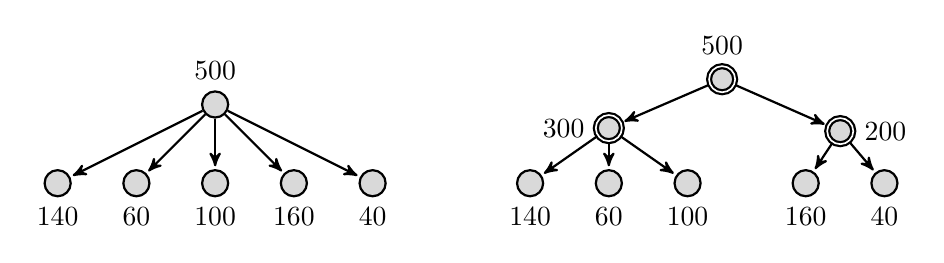
\begin{tikzpicture}[->,>=stealth',shorten >=1pt,auto,node distance=1.cm,
  thick,main node/.style={circle,fill=black!15,draw,font=\sffamily}]

  \node[main node, label=north:500] (1) {};
  \node[main node, label=south:100] (4) [below of=1] {};  
  \node[main node, label=south:60] (3) [left of=4] {};    
  \node[main node, label=south:140] (2) [left of=3] {};  
  \node[main node, label=south:160] (5) [right of=4] {};  
  \node[main node, label=south:40] (6) [right of=5] {}; 

 \node[main node, label=south:140] (7) [right of=6, xshift=1cm] {}; 
 \node[main node, label=south:60] (8) [right of=7] {}; 
 \node[main node, label=south:100] (9) [right of=8] {}; 
 \node[main node, label=south:160] (10) [right of=9, xshift=.5cm] {}; 
 \node[main node, label=south:40] (11) [right of=10] {}; 
  
 \node[main node, yshift=-0.3cm, double,label=west:300] (12) [above of=8] {};
 \node[main node, xshift=.4cm, yshift=-0.3cm, double,label=east:200] (13) [above left = of 11] {};
 \node[main node, xshift=-1.5cm, yshift=-0.7cm, double,label=north:500] (14) [above = of 13] {};
 
  \path[every node/.style={font=\sffamily\tiny}]
    (1) edge node [right] {} (2)
   	    edge node [right] {} (3) 
   	    edge node [right] {} (4)
   	    edge node [right] {} (5)
   	    edge node [right] {} (6)      
    (14) edge node [right] {} (12)
   	     edge node [right] {} (13) 
   	(12) edge node [right] {} (7)
   	     edge node [right] {} (8)
   	     edge node [right] {} (9) 
   	(13) edge node [right] {} (10)
   	     edge node [right] {} (11)      ;
\end{tikzpicture}
\caption{Resource allocation problems can be solved using a hierarchical decomposition structure. Inner nodes representing intermediaries are
marked by double circles.}
\label{fig:hierarchical-decomposition}
\end{figure*}

We present the scheduling problem for some inner node---called intermediary $\AnAvpp$---since the problem is solved top-down, as shown in 
\fref{fig:hierarchical-decomposition}.
Each intermediary in turn redistributes its assigned fraction of the overall demand $\AssResidualLoad{t}{\AnAvpp}$ to 
its subordinate agents $\Subsystem$ until all leaf agents, i.e., physical power plants, are assigned schedules. Note
that the root node $\TlAvpp$ is assigned the actual total demand of the environment, i.e., $\AssResidualLoad{t}{\TlAvpp} = \DemandSym[t]$.
%
\begin{eqnarray}
\label{eq:csop-scheduling-hierarchy} \textstyle
		& \underset{\AgentPower{t}{\AnAgent}}{\operatorname{minimize}} & 
		\alpha_{\ViolationObjective} \cdot \ViolationObjective + \alpha_{\CostsObjective} \cdot \CostsObjective \\
		& \operatorname{subject\ to} & \forall a \in \Subsystem, \forall t \in \Horizon : \exists [x , y] \in \ListProduction{t}\AnAgent : x \leq \AgentPower{t}{\AnAgent} \leq y\text{,} \nonumber \\
		& & \ChangeSpeedMin\AnAgent \left(\AgentPower{t-1}\AnAgent\right) \leq \AgentPower{t}{\AnAgent} \leq \ChangeSpeedMax\AnAgent\left(\AgentPower{t-1}\AnAgent\right) \nonumber\\
		& & \textstyle \text{with } \ViolationObjective = \sum_{t \in \Horizon} \left|\Production_\Subsystem[t] - \AssResidualLoad{t}{\AnAvpp} \right| \text{, } \nonumber \\
		& & \textstyle \text{and } 
		\CostsObjective = \sum_{a \in \Subsystem,\ t \in \Horizon} \CostFunction\AnAgent{\AgentPower{t}{\AnAgent}} \nonumber
\end{eqnarray}
%
We propose to solve this problem using two approaches based on self-organization:
\begin{itemize}
\item A so-called ``regio-central'' approach: agents transfer models to their local supervisor who, at meso-level,
centrally optimizes the allocation~\cite{Schiendorfer2014, SchiendorferSyn2014}
\item An auction-based decentralized approach~\cite{Anders-TAAS-2015}
\end{itemize}

In both cases, obtaining a good abstraction of an intermediary's behavior as a compact
representation of the underlying set of subordinate agents is desirable.

\begin{figure*}
        \centering
        \begin{subfigure}[b]{0.4\textwidth}
        \centering
                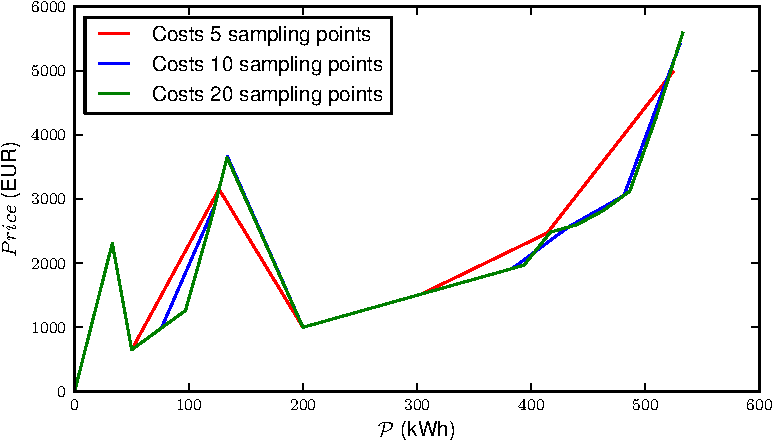
\includegraphics[width=\textwidth]{img/costs}
                \caption{Accuracy affected by the number of sampling points selected.}
                \label{fig:sampling}
        \end{subfigure}%
        ~ \qquad%add desired spacing between images, e. g. ~, \quad, \qquad, \hfill etc.
          %(or a blank line to force the subfigure onto a new line)
        \begin{subfigure}[b]{0.4\textwidth}
        \centering
                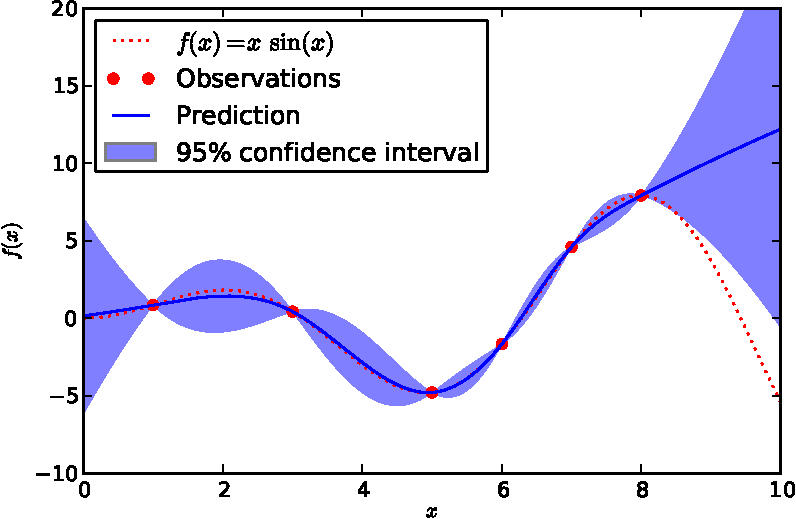
\includegraphics[width=\textwidth]{img/gaussProc}
                \caption{A probabilistic regression model allows to quantify uncertainty at given points in the domain of a learned function.}
                \label{fig:mouse}
        \end{subfigure}
\end{figure*}

%\begin{figure*}
%		\centering
%		 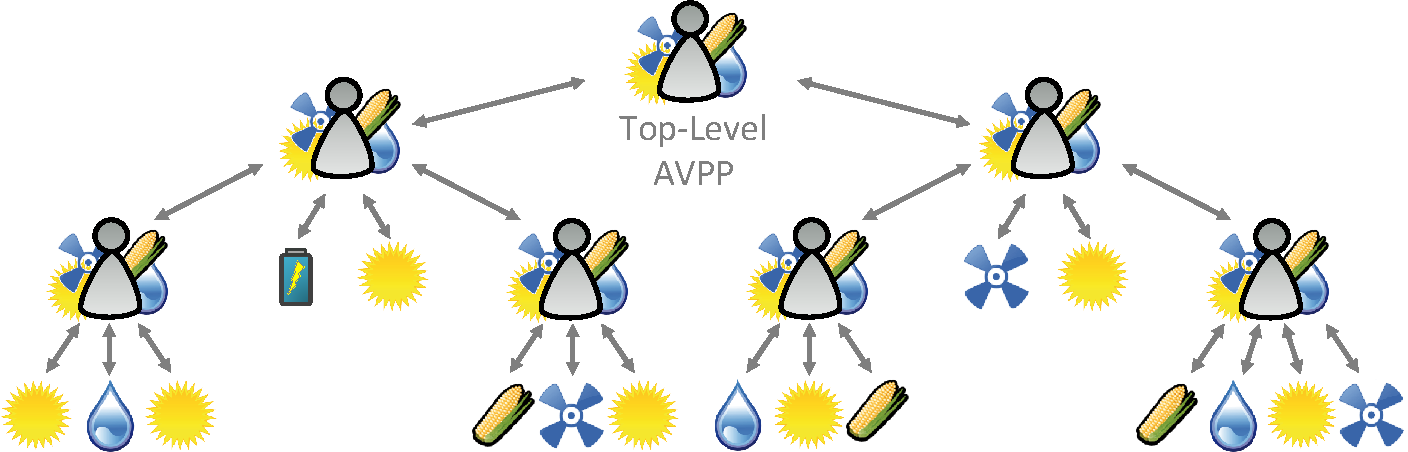
\includegraphics[width=0.55\textwidth]{img/avpp-hierarchical-system-structure.pdf}
%			\caption{Hierarchical system structure of a future autonomous power management system: Prosumers are structured into systems of systems represented by AVPPs acting as intermediaries, thereby decreasing the complexity of control and scheduling. AVPPs can be part of other AVPPs.}
%			%and participate in the power market.}
%		\label{fig:avpp-hierarchical-system-structure}
%\end{figure*}


\section{Obtaining Abstracted Models}

\subsection{Interval Calculations and Sampling Abstraction}

\todo[inline]{This is just copied unpublished material from my thesis, I'll rewrite that.}
In addition to existing abstraction mechanisms that yield constraints shrinking the search space of the production of a virtual agent, we are interested in functional relationships between variables or decision expressions in an SAM. In particular, the maximal production change from one time step to another given the current aggregated production is of interest to improve the accuracy of the AAM. Even though temporal abstraction excludes ranges after t steps, it does not offer any boundaries between two consecutive time steps. A schedule that switches from minimal to maximal production values within the limitations of $\ListSym_t^a$ would be valid according to temporal abstraction but inaccurate given the underlying physical systems' possible inertia. Similarly, a cost function could map the aggregated production to the minimally required cost for a different optimization objective. 

Therefore, we acquire an abstract representation of these functional relationships by \emph{sampling}, i.e., solving several optimization problems and collecting output values. Concretely, these problems consist of the constraints in the SAM and introduce an additional constraint that fixes the input variable to some particular value and tries to minimize or maximize the output variable. For example, $\AgentPower{0}{v}$ (with  $\AgentPower{0}{v}$ still being the sum of all $\AgentPower{0}{a}$) is bound to be $400$ and the objective is to maximize $\AgentPower{1}{v}$.  Then, these input-output pairs can be represented by a suitable approximation method instead. As of now, we employ \emph{piecewise linear functions} that are readily supported by MIP or Constraint Solvers such as CPLEX and have been applied in model abstraction in simulation engineering~\cite{Frantz_Taxonomy}.
%
\begin{algorithm}
\caption{Sampling Abstraction for change speeds}\label{alg:SamplingAbstraction}
\begin{algorithmic}[1]
\Require $(X, D, C)$ is the SAM of $v$
\Ensure $\kappa$ are pairs of the positive change speed
\State $\mathcal{I} \gets s$ sampling points $\in \ListSym^a$
\Procedure{sampling-abstraction}{$v, s$}
\ForAll{$\{i \in \mathcal{I}\}$}
\State $C' \gets C \cup \{(\AgentPower{0}{v} = i)\}$
\State $o \gets $ solve $\langle X, D, C'\rangle$ : $\text{minimize } \CostsObjective[1]$
\State $\kappa \gets \kappa \cup \{(i,o)\}$
\EndFor
\State \textbf{return} $\mathsf{pwLinear}(\kappa)$ 
\EndProcedure
\end{algorithmic}
\end{algorithm}
%
After finding the feasible production ranges of a VA by general abstraction, we can perform sampling abstraction by using a number of sampling points distributed across the production range and collect the respective outputs. Currently these sampling points are selected equidistantly across the full range. We sketch the approach in \aref{alg:SamplingAbstraction} for the positive production change speed. The ``sampled'' piecewise linear function can then be used for additional constraints in the AAM .
\subsection{Modifying existing SCSOPs for sampling Input-Output pairs}
Given that the agent models are already available in a constraint language as needed for the load distribution problem, the main idea in sampling consists of reusing these constraints and formulating new problems. Compared to the distribution model, no residual load or initial states are included in these ``sampling'' models. A special role is given to the decision variables for the agents' production at time step 0. Usually constraints link the current state to these variables, e.g. $\AgentPower{0}{a} = 10.0$. But in this case these constraints are dropped and an additional constraint only ensures that a suitable initial state is found which is bound to an aggregate value: $\sum_{a \in \Subsystem} \AgentPower{0}{a} = 500.0$. Then a suitable valuation for the productions at $0$ are sought by the solver and a target expression is maximized or minimized.

\subsection{Piecewise Linear Functions for Sampled Functions}

\begin{figure*}
        \centering
        \begin{subfigure}[b]{0.4\textwidth}
      \centering
      	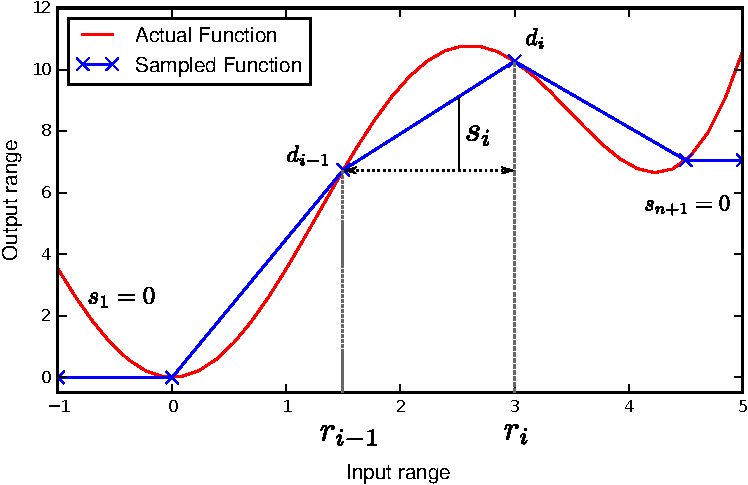
\includegraphics[width=\textwidth]{img/piecewiselin.pdf}
      	\caption{Example function $f(x) = x^2 + 3 x \sin(x)$ sampled at $\{0, 1.5, 3.0, 4.5\}$.  }
      	\label{fig:pwlFunction}
        \end{subfigure}%
        ~ \qquad%add desired spacing between images, e. g. ~, \quad, \qquad, \hfill etc.
          %(or a blank line to force the subfigure onto a new line)
        \begin{subfigure}[b]{0.4\textwidth}
        \centering
        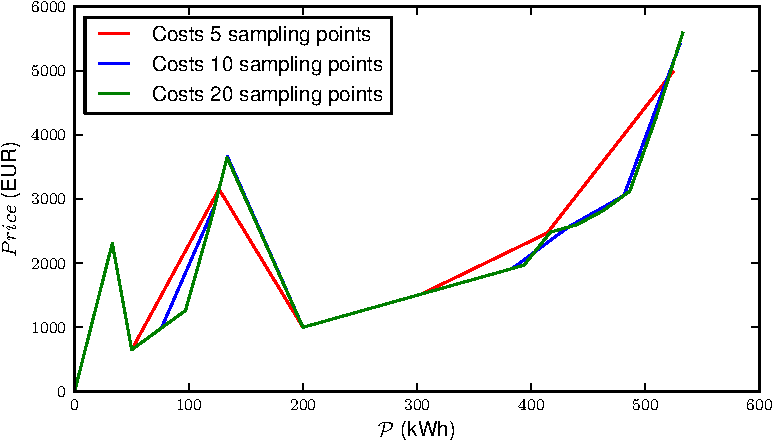
\includegraphics[width=\textwidth]{img/costs.pdf}
        \caption{Cost function sampled at different accuracies }
        \label{fig:costsFunction}
        \end{subfigure}
\end{figure*}

\subsection{Sampling Change Functions for an Abstracted Agent Model}
The following graphs illustrate what piecewise linear approximations of functions of decision expressions in synthesized regional models look like for the AVPP example presented in \sref{sec:runningExample}. We revisit the virtual agent $w$ consisting of three concrete agents:
%
\begin{description}
\item[a:] $\ListSym^a = \langle [0,0], [50, 100] \rangle$, $\gamma^a = 13$
\item[b:] $\ListSym^b = \langle [0,0], [15, 35] \rangle$, $\gamma^b = 70$
\item[c:] $\ListSym^c = \langle [0,0], [200, 400] \rangle$, $\gamma^c = 5$
\end{description}
where $\gamma$ is the price per production unit such that the total cost for one time step is given by $\sum_{a' \in \{a,b,c\}} \gamma^{a'} \AgentPower{t}{a'}$. General abstraction gave the feasible production space of this virtual agent in \sref{sec:generalAbstraction}: $\ListSym^v = \langle [0.0 0.0], [15.0 35.0], [50.0 135.0], [200.0 535.0] \rangle$. Different numbers of sampling points are selected equidistantly over the whole production space in addition to the boundary points of the intervals. Therefore, the more sampling points are used the higher the accuracy of the obtained piecewise linear function.


The objective for the function in \fref{fig:costsFunction} was set to minimize the cost given a combined production. As in this example low production rates are set to be quite expensive, also the combined production of the virtual agent is more expensive at low rates.

\subsection{Issues with Sampling Abstraction}
However, if
the selected input-output pairs are selected in a weakly informative way, the resulting abstracted
optimization problem introduces severe errors in quality as well as bad runtime performance.


\section{Improving Sampling Point Selection by Active Learning}
\todo[inline]{Just some very preliminary pointers to literature}
Active learning using Gaussian process has been applied to several problems~\cite{Krause2007,Krause2008,Park2011}. 

\section{Evaluation}
We investigate the effects of selecting a particular set of 
sampling points for one group that could have emerged as part
of a self-organization process.


%\section*{Acknowledgment}
%This research is partly sponsored by the research unit \emph{OC-Trust} (FOR 1085) of the German Research Foundation.

\bibliographystyle{IEEEtran}
\bibliography{saos}

\end{document}
